% Camera-ready · Beschäftigungstiefe Schönefeld · für Thomas Graf (Alpine Immobilien)
% Build: pdflatex graf-beschaeftigung-thomas-graf-de.tex  (2×)
%        oder: npm run graf:report:de

\documentclass[11pt,a4paper,ngerman]{scrartcl}

\usepackage[utf8]{inputenc}
\usepackage[T1]{fontenc}
\usepackage{lmodern}
\usepackage{microtype}
\usepackage{geometry}
\geometry{left=2.4cm,right=2.4cm,top=2.6cm,bottom=2.8cm,headheight=14pt}

\usepackage{graphicx}
\usepackage{booktabs}
\usepackage{tabularx}
\usepackage{caption}
\usepackage{subcaption}
\usepackage{xcolor}
\usepackage{hyperref}
\usepackage{fancyhdr}
\usepackage{enumitem}
\usepackage[ngerman]{babel}
\usepackage[autostyle=true]{csquotes}

\definecolor{berblue}{HTML}{1e3a5f}
\definecolor{bergold}{HTML}{b45309}

\hypersetup{
  colorlinks=true,
  linkcolor=berblue,
  urlcolor=berblue,
  pdfauthor={BER+ Board Room · IDI S26},
  pdftitle={Beschäftigungstiefe nahe Schönefeld — Briefing für Thomas Graf}
}

\graphicspath{{figures/}}
\captionsetup{font=small,labelfont=bf,skip=6pt}
\setlist[itemize]{noitemsep,topsep=0.25em,parsep=0pt}
\setlist[enumerate]{noitemsep,topsep=0.25em,parsep=0pt}

\newcommand{\berhub}{\textbf{BER+ Board Room}}
\newcommand{\indikativ}{\textit{Indikative Auswertung — keine amtliche Arbeitsmarktstatistik}}

\pagestyle{fancy}
\fancyhf{}
\fancyhead[L]{\small\color{black!55}Beschäftigungstiefe · Schönefeld-Korridor}
\fancyhead[R]{\small\color{black!55}\berhub}
\fancyfoot[C]{\small\thepage}
\renewcommand{\headrulewidth}{0.4pt}
\renewcommand{\footrulewidth}{0pt}

\begin{document}

% --- Titelseite ---
\begin{titlepage}
  \centering
  \vspace*{1.2cm}
  {\color{berblue}\rule{\linewidth}{1.2pt}}\\[0.8em]
  {\LARGE\bfseries Beschäftigungstiefe nahe Schönefeld}\\[0.35em]
  {\large Arbeitskräfte- und Mieterpotenzial für Büro- und Gewerbeprojekte}\\[1.2em]
  {\normalsize\indikativ}\\[2em]

  \begin{minipage}{0.82\linewidth}
    \centering
    {\large\textbf{Kurzbriefing für}}\\[0.4em]
    {\Large Thomas Graf}\\[0.2em]
    {\normalsize Geschäftsführer, Alpine Immobilien GmbH\\
    2.\ Vorsitzender, \textit{Berlin Airports Region Plus e.\,V.} (BER+)\\
    Referenzprojekt: BB Business Hub, Schönefeld}
  \end{minipage}

  \vfill
  {\normalsize Erstellt im Rahmen des IDI-Projekts S26 (2026)}\\[0.3em]
  {\small XU University of Applied Sciences · Tian Shao · Yushu Qin · Yi Li}\\[0.8em]
  {\small Juni 2026 · Datenstand: OpenStreetMap / öffentliche Quellen}\\[0.5em]
  {\color{berblue}\rule{\linewidth}{1.2pt}}
\end{titlepage}

\thispagestyle{empty}
\section*{Zusammenfassung}
\addcontentsline{toc}{section}{Zusammenfassung}

Nach der BER+-Präsentation im Juni 2026 haben Sie die Frage gestellt, ob die Unternehmen nahe Schönefeld genügend Beschäftigte haben, damit neue \textbf{Büro- und Gewerbeflächen} erfolgreich vermietet werden können.

\textbf{Kernantwort.} Die Frage ist weniger eine Frage nach \enquote{Bauarbeiterzahl} vor Ort als nach \textbf{Beschäftigungstiefe}: Wie viele Firmen und Arbeitsplätze existieren bereits im Korridor? Können neue Mieter \textbf{Fachkräfte} aus dem Einzugsgebiet Berlin–Brandenburg gewinnen?

\textbf{Vorgehen.} Wir haben \textbf{215 benannte Arbeitgeber} aus Live-OpenStreetMap-Daten (Schönefeld-Bbox) kartiert, öffentlich verfügbare Beschäftigtenzahlen abgeglichen und für verbleibende Standorte ein \textbf{transparentes Korridor-Beschäftigungsmodell} angewendet. Die Auswertung ist im \berhub{} unter \url{https://ber-board-room.vercel.app/beschaeftigung} eingebunden.

\textbf{Leitbefunde (indikativ).}
\begin{itemize}
  \item \textbf{BB Business Hub} (Ihr Campus-Referenz): ca.\ 50 Firmen, ca.\ 800 Beschäftigte (Mitgliedermeldung Alpine / BER+, Feb.\ 2025).
  \item \textbf{Flughafen Berlin Brandenburg GmbH (FBB):} ca.\ 2{,}131 Beschäftigte (Jahresdurchschnitt 2023, Geschäftsbericht).
  \item \textbf{643} Gewerbe- und Industrieobjekte in OSM; davon \textbf{215} mit Firmennamen.
  \item \textbf{102} Standorte ohne öffentliche Standortzahl — modelliert mit Summe ca.\ \textbf{4{,}075} Planungswerten.
  \item \textbf{Korridor-Fußabdruck} (Standort- + Modell- + Mikroschätzungen, \textit{ohne} Konzern-HQ-Zahlen wie DHL global): Größenordnung ca.\ \textbf{15{,}000} Arbeitsplätze als plausible lokale Präsenz.
\end{itemize}

\textbf{Empfehlung.} Briefing auf der neutralen Board-Room-Karte veröffentlichen; \textbf{90-Tage-Mitgliedervalidierung} mit Alpine und 3–5 Anker-Mitgliedern, bevor Vermietungsnarrative als belastbar gelten.

\tableofcontents
\newpage

\section{Ausgangslage und Fragestellung}
\label{sec:frage}

Ihr Referenzprojekt \textbf{BB Business Hub} zeigt, dass ein multi-tenant-fähiger Gewerbestandort Dutzende Firmen und Hunderte Arbeitsplätze tragen kann. Für neue Alpine-Projekte im Schönefelder Korridor stellt sich die strategische Frage: Wie vergleicht sich diese Tiefe mit dem übrigen Gewerbeband?

\begin{figure}[htbp]
  \centering
  
\includegraphics[width=\linewidth,keepaspectratio]{fig-app-hero.png}
  \caption{Stakeholder-Signal im \berhub{} — Umdeutung der \enquote{Manpower}-Frage als Beschäftigungstiefe (Screenshot \texttt{/beschaeftigung}).}
\end{figure}

\begin{quote}
  \emph{\enquote{Employieren die Firmen nahe Schönefeld genug Menschen — wird ein neues Büro/Gewerbe-Projekt Mieter und Fachkräfte finden?}}
\end{quote}

\section{Einordnung: Beschäftigungstiefe statt Baustellenlogik}
\label{sec:reframe}

\begin{figure}[htbp]
  \centering
  \begin{subfigure}[t]{0.48\textwidth}
    \centering
    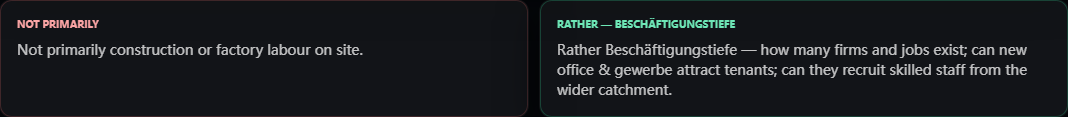
\includegraphics[width=\linewidth,keepaspectratio]{fig-app-reframe.png}
    \caption*{Nicht primär: Bau- oder Fabrikpersonal}
  \end{subfigure}\hfill
  \begin{subfigure}[t]{0.48\textwidth}
    \centering
    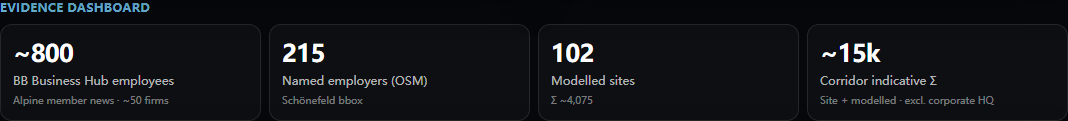
\includegraphics[width=\linewidth,keepaspectratio]{fig-app-dashboard.png}
    \caption*{Evidenz-Dashboard}
  \end{subfigure}
  \caption{Neuinterpretation und Kennzahlenübersicht.}
\end{figure}

\begin{description}[style=nextline,leftmargin=2.8cm,font=\normalfont\bfseries]
  \item[Nicht primär] Bau- oder Fabrikarbeitskräfte direkt auf dem Grundstück.
  \item[Sondern] \textbf{Beschäftigungstiefe} — Mieterstruktur, bestehende Jobs im Korridor, Rekrutierbarkeit von Fachkräften aus dem Metropolraum (ca.\ 6\,Mio.\ Einwohner Berlin–Brandenburg).
\end{description}

Die Flughafenregion-Studie (FBB / WFBB / IHK, 2025) benennt \textbf{Fachkräftegewinnung} als zentrale Herausforderung — nicht fehlende Arbeitskräfte generell.

\section{Daten und Evidenz auf einer Karte}
\label{sec:daten}

\begin{figure}[htbp]
  \centering
  
\includegraphics[width=\linewidth,height=0.34\textheight,keepaspectratio]{fig-app-map.png}
  \caption{Live-OSM-Gewerbeschicht — 643 Objekte; benannte Arbeitgeber hervorgehoben; Anker BB Business Hub.}
\end{figure}

{\small
\begin{tabularx}{\linewidth}{@{}p{3.1cm}Xp{1.5cm}@{}}
\toprule
\textbf{Datenschicht} & \textbf{Geschäftliche Bedeutung} & \textbf{Anz.} \\
\midrule
OSM-Gewerbeobjekte & Physische Präsenz wirtschaftlicher Aktivität & 643 \\
Benannte Arbeitgeber & Mit Mitgliedern diskutierbare Firmen / Standorte & 215 \\
Verifiziert (Standort / Register) & Zitierfähige Zahlen für Vorstand / Leasing & 9 \\
Konzern-Markenmatch & Marke vor Ort; HQ-Zahl \textit{nicht} lokale Beschäftigung & 53 \\
Modellierte Standorte & Transparente Schätzung ohne öffentliche Meldung & 102 \\
Mikro-Einheiten & Dienstleistung / Einzelhandel (nur Spannen) & 51 \\
\bottomrule
\end{tabularx}
}

\section{Korridor-Beschäftigungsmodell}
\label{sec:modell}

\textit{Zweck:} Eine verteidigbare \textbf{Erstantwort} liefern, wo öffentliche Daten enden — ohne vertrauliche HR-Unterlagen vorzutäuschen.

\textbf{Dreistufige Logik (keine Blackbox).}
\begin{enumerate}
  \item \textbf{Veröffentlichtes zuerst.} Geschäftsberichte, Mitgliedernews (BB Hub), Registerauszüge (FBB) verankern die Erzählung.
  \item \textbf{Standort nach Betriebstyp klassifizieren.} Logistik, Werkstätten, Gewerbeparks, Flughafengebäude, Einzelhandel — angelehnt an Mittelstandstruktur (viele kleine, wenige große Betriebe).
  \item \textbf{Korridor-Kontext.} Nähe zu BER erhöht die angenommene Beschäftigungsdichte moderat — konsistent mit der regionalen Arbeitsmarktlage.
\end{enumerate}

\textbf{Ausgabeformat.} Für jeden der 102 nicht gemeldeten Standorte: \textbf{Spanne} (konservativ–optimistisch) und ein \textbf{Planungswert} innerhalb der Spanne.

\begin{center}
{\small
\begin{tabular}{lrr}
\toprule
\textbf{Standort (OSM-Name)} & \textbf{Planungswert} & \textbf{Spanne} \\
\midrule
Gewerbepark Schönefeld & 357 & 92--402 \\
Logistikzentrum Airport Park Berlin & 192 & 69--253 \\
Briefzentrum 12 / Logistikzentrum Berlin Südost & 171 & 69--253 \\
Berlin ExpoCenter Airport & 123 & 29--161 \\
\bottomrule
\end{tabular}
}
\end{center}

{\small Vollständige 102-Zeilen-Tabelle: \texttt{public/data/graf/employee-predictions.json} und interaktive Oberfläche im \berhub{}.}

\begin{figure}[htbp]
  \centering
  \begin{subfigure}[t]{0.48\textwidth}
    \centering
    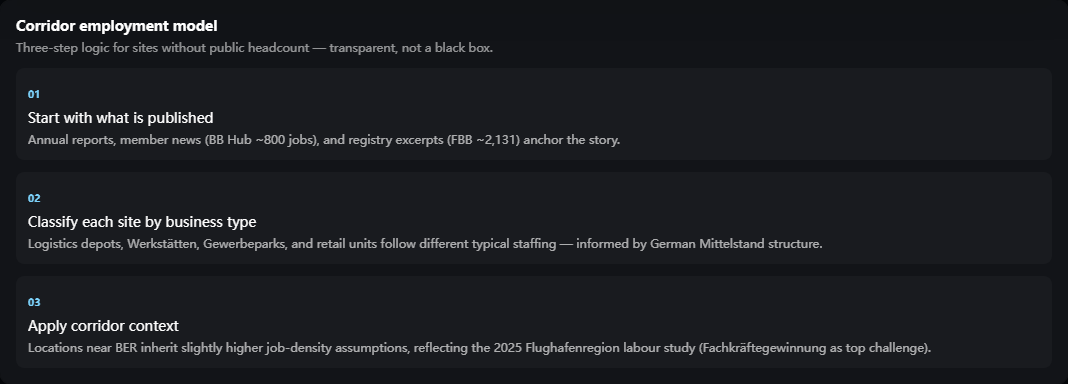
\includegraphics[width=\linewidth,keepaspectratio]{fig-app-model.png}
    \caption*{Modell in drei Schritten}
  \end{subfigure}\hfill
  \begin{subfigure}[t]{0.48\textwidth}
    \centering
    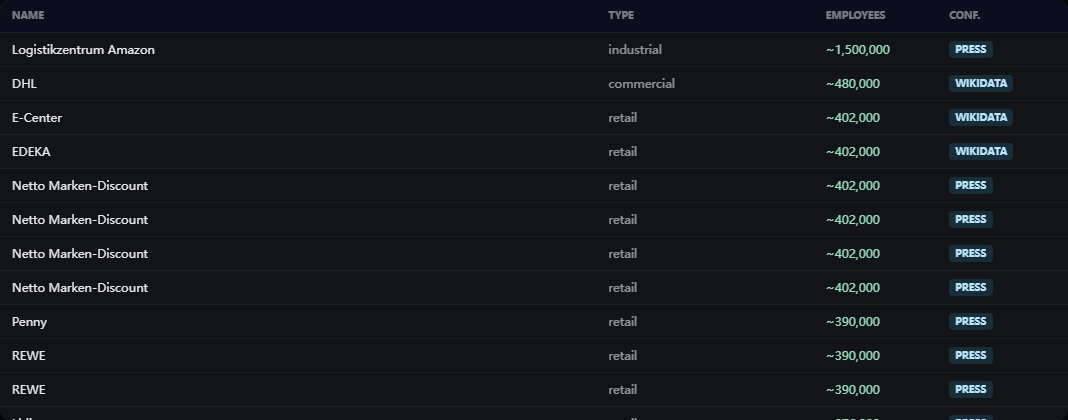
\includegraphics[width=\linewidth,keepaspectratio]{fig-app-table.png}
    \caption*{Arbeitgeber-Abgleichtabelle}
  \end{subfigure}
  \caption{Modellerklärung und durchsuchbare Tabelle mit Konfidenzkennzeichnung.}
\end{figure}

\textbf{Bewusst ausgeschlossen.}
\begin{itemize}
  \item DHL / REWE / Amazon-\textbf{Konzern}-Beschäftigtenzahlen als Schönefeld-Standortpersonal summieren.
  \item Modellwerte als geprüfte Beschäftigtenzahlen ausweisen.
  \item Mitgliedervalidierung durch ein GIS ersetzen.
\end{itemize}

\section{Antwort für Alpine und den BER+-Vorstand}
\label{sec:antwort}

\textbf{Reicht die \enquote{Manpower}?}
\begin{itemize}
  \item \textbf{Ja für narrative Glaubwürdigkeit:} Hunderte benannter Gewerbestandorte, validierter Flughafenarbeitgeber (FBB ca.\ 2\,k), eigener BB-Hub-Beleg (ca.\ 800).
  \item \textbf{Mit Vorbehalten für Leasing:} Mietergewinnung hängt von \textbf{Fachkräfte-Mobilität} im Metropolraum ab — nicht nur von lokal gemessener Kopfzahl.
  \item \textbf{Nächster Glaubwürdigkeitsschritt:} mitgliederbestätigte Firmenzahlen für Pilot-1 und 3–5 Anker (Alpine, SEGRO, BUWOG, WFG, Sector Seven).
\end{itemize}

\section{Integration im \berhub{} und Pilotvorschlag}
\label{sec:pilot}

Die finale Version ist in die Next.js-Hauptanwendung integriert — erreichbar über die Fußzeilen-Navigation \textit{Workforce} und die Briefing-Karte.

\begin{figure}[htbp]
  \centering
  \begin{subfigure}[t]{0.48\textwidth}
    \centering
    
\includegraphics[width=\linewidth,keepaspectratio]{fig-app-board-briefing-tab.png}
    \caption*{Briefing-Tab im War-Room}
  \end{subfigure}\hfill
  \begin{subfigure}[t]{0.48\textwidth}
    \centering
    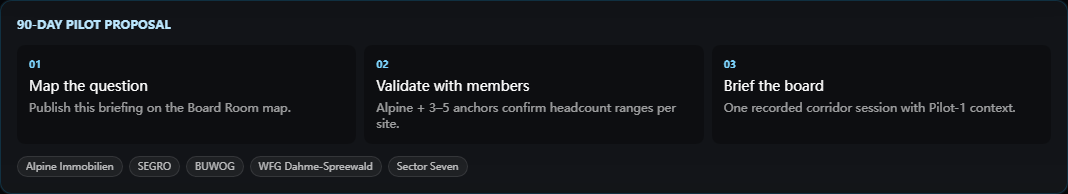
\includegraphics[width=\linewidth,keepaspectratio]{fig-app-pilot.png}
    \caption*{90-Tage-Pilot}
  \end{subfigure}
  \caption{Navigation im Board Room und vorgeschlagener Validierungspfad.}
\end{figure}

\textbf{90-Tage-Pilot (Vorschlag).}
\begin{enumerate}
  \item \textbf{Frage kartieren} — Briefing auf der neutralen Board-Room-Karte veröffentlichen.
  \item \textbf{Mit Mitgliedern validieren} — Alpine plus 3–5 Anker bestätigen Beschäftigungsspannen je Standort.
  \item \textbf{Vorstand briefen} — eine aufgezeichnete Korridor-Sitzung mit Pilot-1-Kontext.
\end{enumerate}

\section{Quellen und Grenzen}
\label{sec:quellen}

\textbf{Quellen:} OpenStreetMap / Overpass (Schönefeld-Bbox, Juni 2026); Alpine / BER+-Mitgliedernews (BB Business Hub); FBB Geschäftsbericht 2023; FBB/WFBB/IHK Arbeitsmarktstudie Flughafenregion 2025; Jahresberichte / Wikidata nur für Markenreferenzen.

\textbf{Grenzen:} OSM-Tags $\neq$ Beschäftigtenzahlen; Modelloutput sind Planungsschätzungen; doppelte OSM-Knoten für dieselbe Anlage können getrennt gezählt sein; vor Veröffentlichung Mitglieder-Workshop empfohlen.

\vspace{1em}
\noindent{\color{black!35}\rule{\linewidth}{0.4pt}}
\vspace{0.5em}

{\small
\noindent\textbf{Ansprechpartner Projekt:} IDI S26 · \berhub{}\\
\textbf{Interaktive Karte:} \url{https://ber-board-room.vercel.app/beschaeftigung}\\
\textbf{Datenpipeline:} \texttt{demos/graf-beschaeftigung-briefing/} $\rightarrow$ \texttt{public/data/graf/}
}

\end{document}
